\textbf{\underline{\large{1.5: Intro to AP: Basic Derivatives Numerically and Graphically}}} \par

Traditionally, calculus was an algebraically heavy subject. One of the philosophical changes that the CollegeBoard made in the 1990s was to emphasize that calculus should be understood in a variety of modes. As they state in their enduring understanding: \begin{center}
    \parbox{0.8\textwidth}{\textit{
        ``Students should be able to work with functions represented in a veriety of ways: graphical, numerical, analytical or verbal.  They should understand the connections among these representations.''}
    }
\end{center} \par

Later, they added that students should be able to verbalize their understanding and be able to communicate that understanding through proper writing. We will consider this later as we consider more context-oriented problems. \par

\begin{tcolorbox}[objective]
    \begin{center}
        OBJECTIVES \\[11pt]
    \end{center}
    Determine Derivative Values from Numerical or Graphical Data.
\end{tcolorbox} \vspace{11pt}

\begin{tcolorbox}[example]
    \textbf{Ex 1.5.1: } Assume $h(x) = f(x)g(x)$. Given the table of values below, find $h'(2)$. \begin{align*}
        \arraycolsep=11pt\def\arraystretch{2.2}
        \begin{array}{|c|c|c|c|c|}
            \hline
            x & f(x) & g(x) & f'(x) & g'(x) \\[11pt] \hline
            1 & 3 & 2 & 4 & 6 \\[5.5pt] \hline
            2 & 1 & 8 & 5 & 7 \\[5.5pt] \hline
            3 & 7 & 2 & 7 & 9 \\[5.5pt]
            \hline
        \end{array}
    \end{align*}
\end{tcolorbox}
\begin{tcolorbox}[solution]
    \textbf{Sol 1.5.1: } \begin{align*}
        & h(x) = f(x)g(x) \\[11pt]
        & h'(x) = f(x)g'(x) + g(x)f'(x) \\[11pt]
        & h'(2) \begin{aligned}[t]
            & = f(2)g'(2) + g(2)f'(2) \\[11pt]
            & = 1 \cdot 7 + 8 \cdot 5 \\[11pt]
            & = \boxed{47}
        \end{aligned}
    \end{align*}
\end{tcolorbox} \vspace{11pt}

\begin{tcolorbox}[example]
    \textbf{Ex 1.5.2: } Using the table of values in \textbf{Ex 1.5.1:}, find $\diff \left[f(g(x))\right]$ and $\diff \left[g(f(x))\right]$ at $x = 1$. 
\end{tcolorbox}
\begin{tcolorbox}[solution]
    \textbf{Sol 1.5.2: } These are two different but similar problems, so let's consider them individually. \begin{align*}
        & \diff \left[f(g(x))\right] \eval_{x = 1} \begin{aligned}[t]
            & = f'(g(1)) \cdot g'(1) \\[11pt]
            & = f'(2) \cdot 6 \\[11pt]
            & = 5 \cdot 6 \\[11pt]
            & = \boxed{30}
        \end{aligned}
    \end{align*} \begin{align*}
        & \diff \left[g(f(x))\right] \eval_{x = 1} \begin{aligned}[t]
            & = g'(f(1)) \cdot f'(1) \\[11pt]
            & = g'(3) \cdot 4 \\[11pt]
            & = 9 \cdot 4 \\[11pt]
            & = \boxed{36}
        \end{aligned}
    \end{align*}
\end{tcolorbox} \vspace{11pt}

\begin{tcolorbox}[example]
    \textbf{Ex 1.5.3: } Given the graph below, find (a) $w'(1)$ if $w = \dfrac{g(x)}{f(x)}$ and (b) $v'(1)$ if $v = g(f(x))$. \\

    \begin{center}
        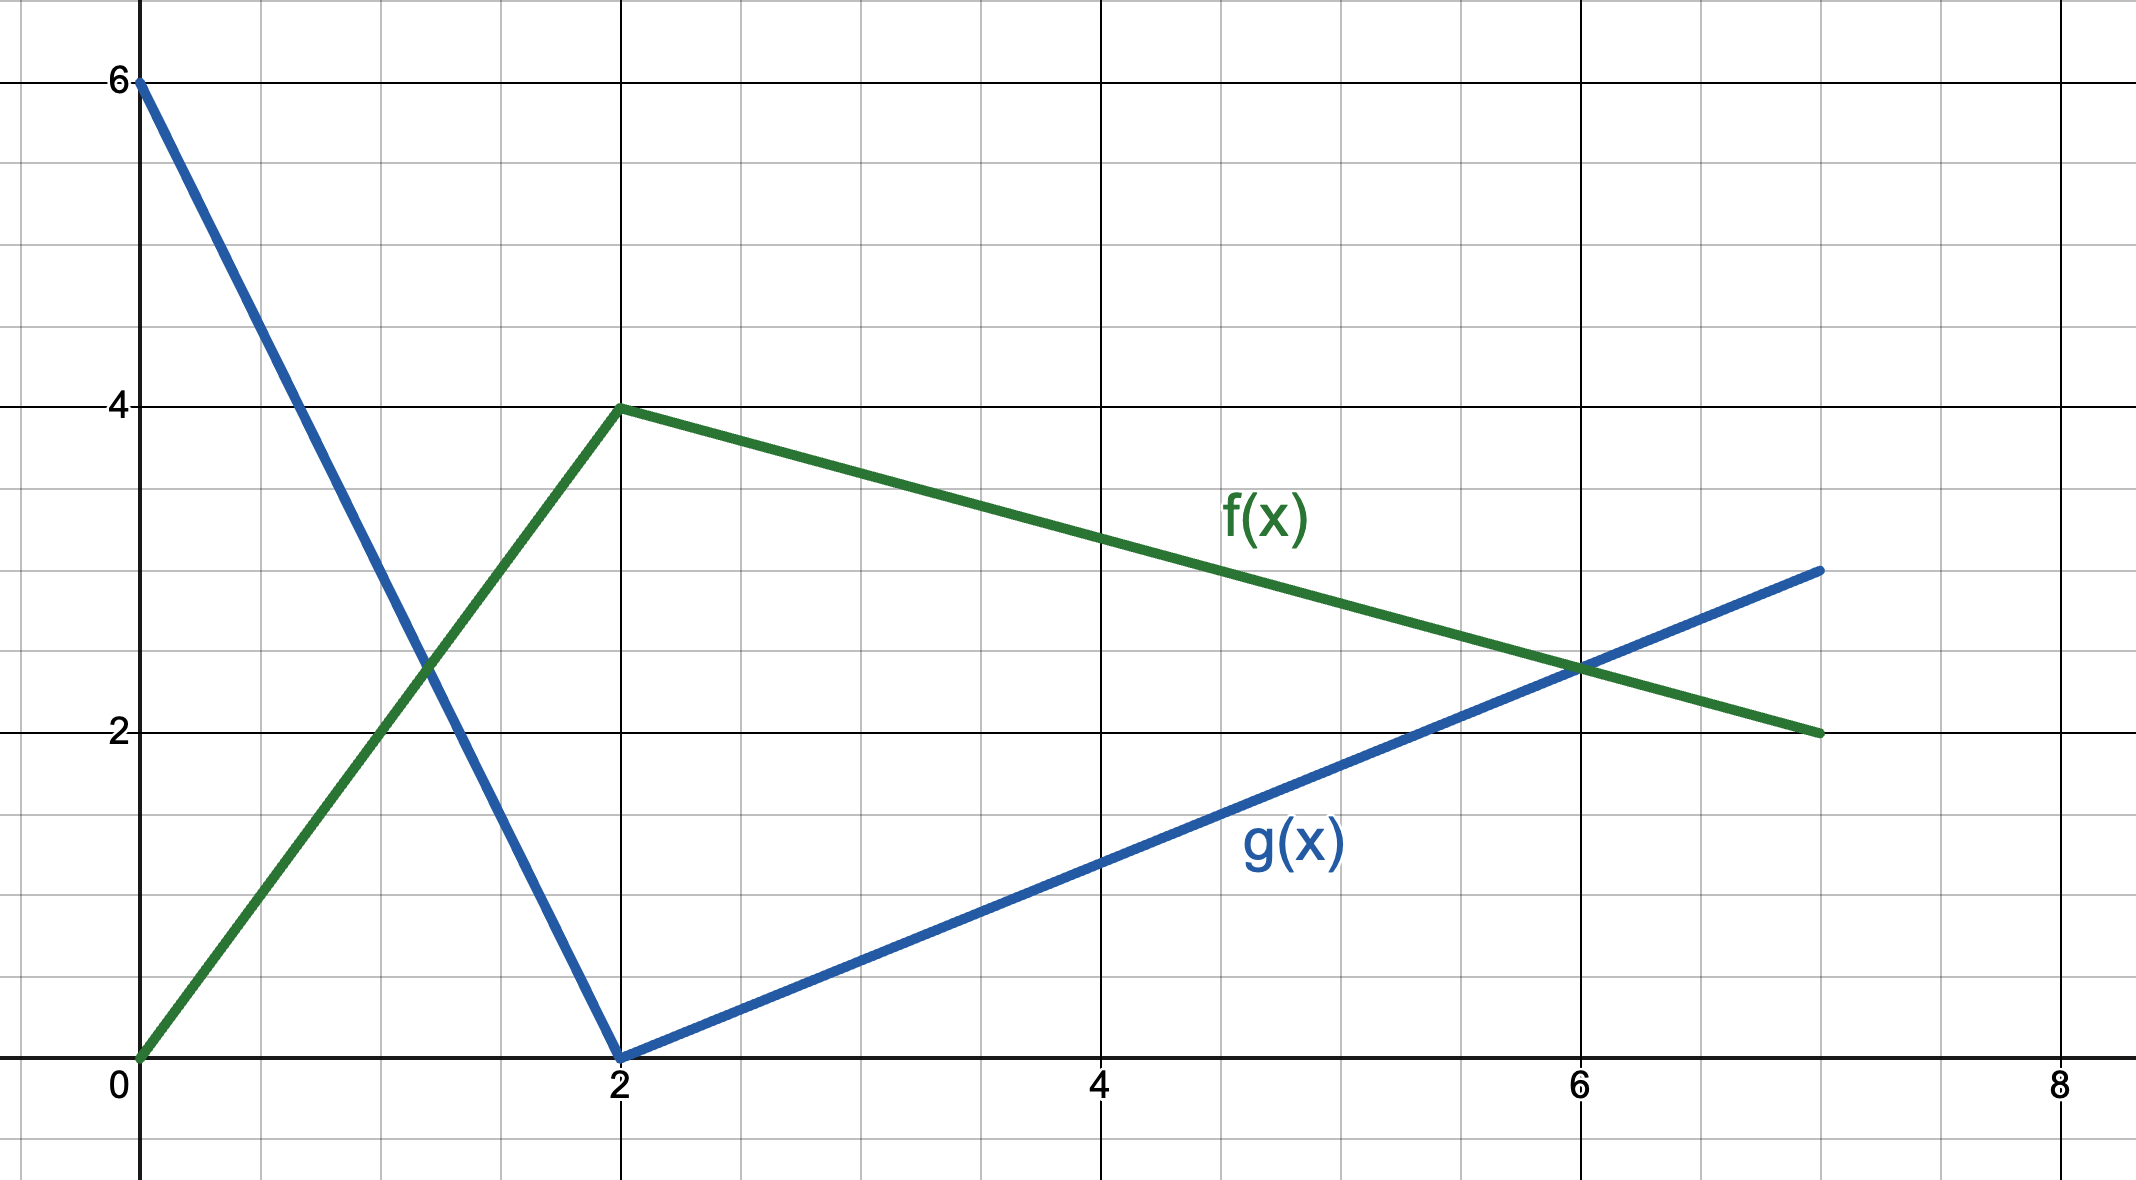
\includegraphics[width = 0.75\textwidth]{Support/Chapter 1 Graphics/1.5-Graphic1.png}
    \end{center}
\end{tcolorbox}
\begin{tcolorbox}[solution]
    \textbf{Sol 1.5.3: } \\[11pt]
    (a) \begin{align*}
        & w = \dfrac{g(x)}{f(x)} \therefore w' = \dfrac{f(x)g'(x) - g(x)f'(x)}{[f(x)]^2} \\[11pt]
        & w'(1) \begin{aligned}[t]
            & = \dfrac{f(1)g'(1) - g(1)f'(1)}{[f(1)]^2} \\[11pt]
            & = \dfrac{2 \cdot (-3) - 3 \cdot 2}{2^2} \\[11pt]
            & = \boxed{-3}
        \end{aligned}
    \end{align*}
    (b) \begin{align*}
        & v(x) = g(f(x)) \\[11pt]
        & v'(x) = g'(f(x)) \cdot f'(x) \\[11pt]
        & v'(1) \begin{aligned}[t]
            & = g'(f(1)) \cdot f'(1) \\[11pt]
            & = g'(2) \cdot 2 \\[11pt]
            & = \boxed{DNE}
        \end{aligned}
    \end{align*}
    (Note that $g'(2)$ does not exist. The slope cannot be determined at $x = 1$ because the slopes to the left and right of $x = 1$ are different. The is called a corner point, or a cusp point, and will be explored further in a later chapter.)
\end{tcolorbox} \vspace{11pt}

\begin{tcolorbox}[example]
    \textbf{Ex 1.5.4: } The figure below shows the graph of the functions $f$ and $g$. The graphs of the lines tangent to the graph of $f$ at $x = -2$ and $x = 1$ are also shown. If $B(x) = f(x) \cdot g(x)$, what is $B'(1)$? \\

    \begin{center}
        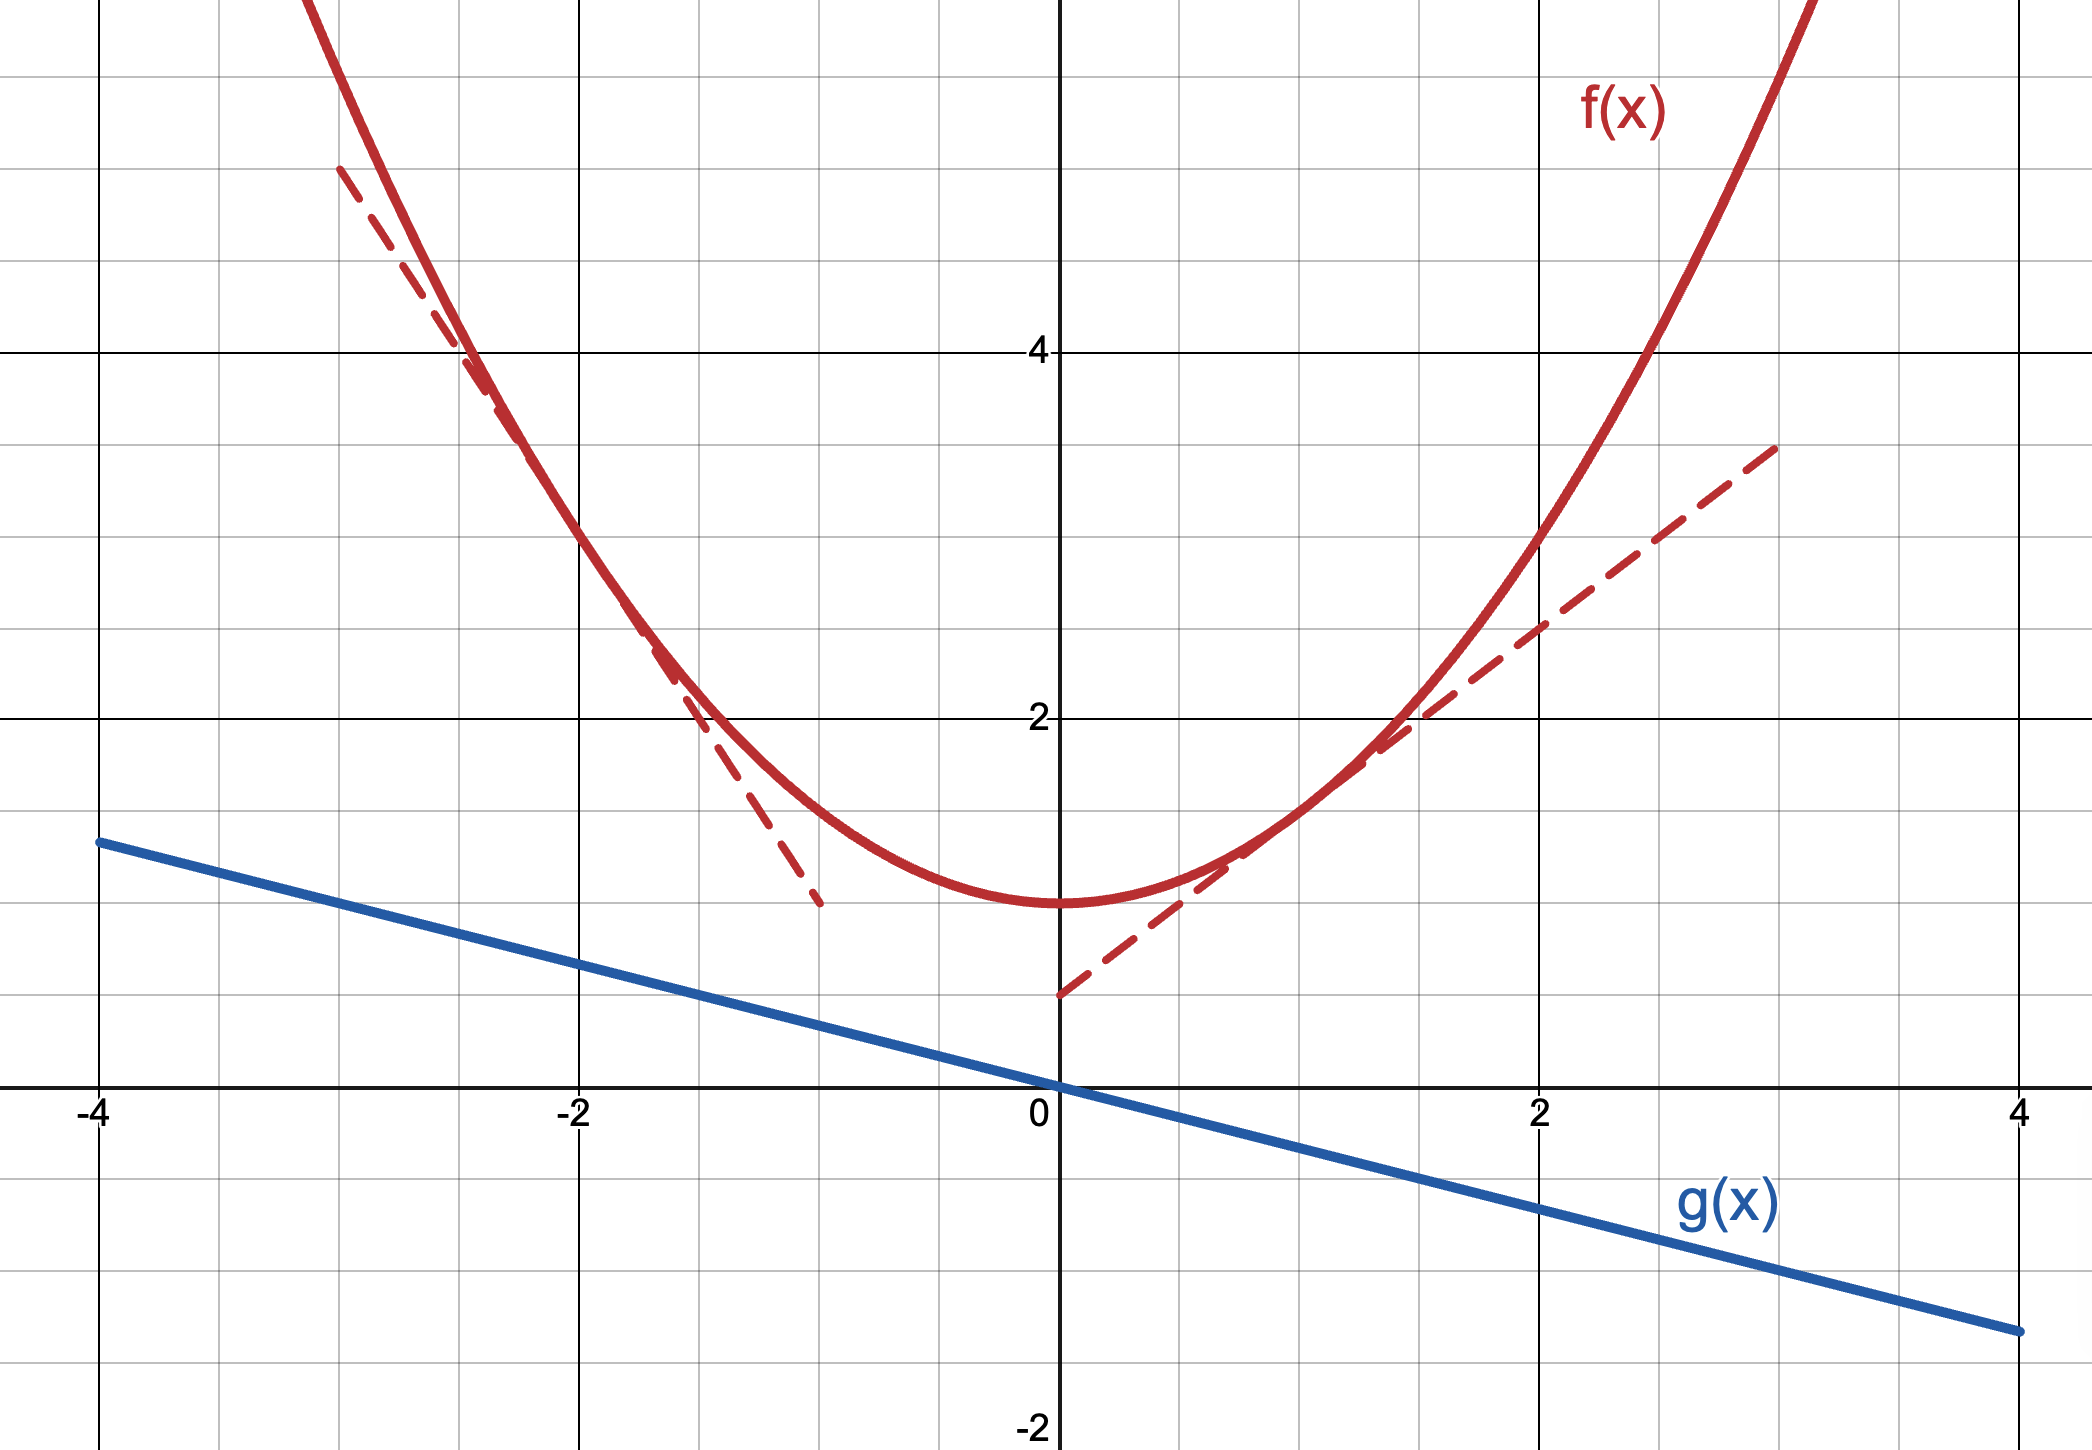
\includegraphics[width = 0.75\textwidth]{Support/Chapter 1 Graphics/1.5-Graphic2.png}
    \end{center} \vspace{11pt}

    \begin{oneparchoices}
        \choice $-\dfrac{5}{6}$
        \choice $-\dfrac{1}{2}$
        \choice $\dfrac{1}{6}$
        \choice $\dfrac{1}{3}$
        \choice $\dfrac{1}{2}$
    \end{oneparchoices}
\end{tcolorbox}
\begin{tcolorbox}[solution]
    \textbf{Sol 1.5.4: } \begin{align*}
        & B(x) = f(x) \cdot g(x) \\[11pt]
        & B'(x) = f(x)g'(x) + g(x)f'(x) \\[11pt]
        & B'(1) \begin{aligned}[t]
            & = f(1)g'(1) + g(1)f'(1) \\[11pt]
            & = \dfrac{3}{2} \cdot \left(-\dfrac{1}{3}\right) + \left(-\dfrac{2}{3}\right) \cdot 1 \\[11pt]
            & = \boxed{\text{a) } -\dfrac{5}{6}}
        \end{aligned}
    \end{align*}
\end{tcolorbox} \vspace{11pt}

\begin{tcolorbox}[example]
    \textbf{Ex 1.5.5: } Let $f(x)$ be the function whose graph is given below and let $g(x)$ be a differentiable function with selected values for $g(x)$ and $g'(x)$ given in the table below. Furthermore, let $h$ be the function defined by $h(x) = \ln \left(x^2 + 4\right)$. \\
    \begin{minipage}[t]{0.75\textwidth} \vspace{0pt}%
        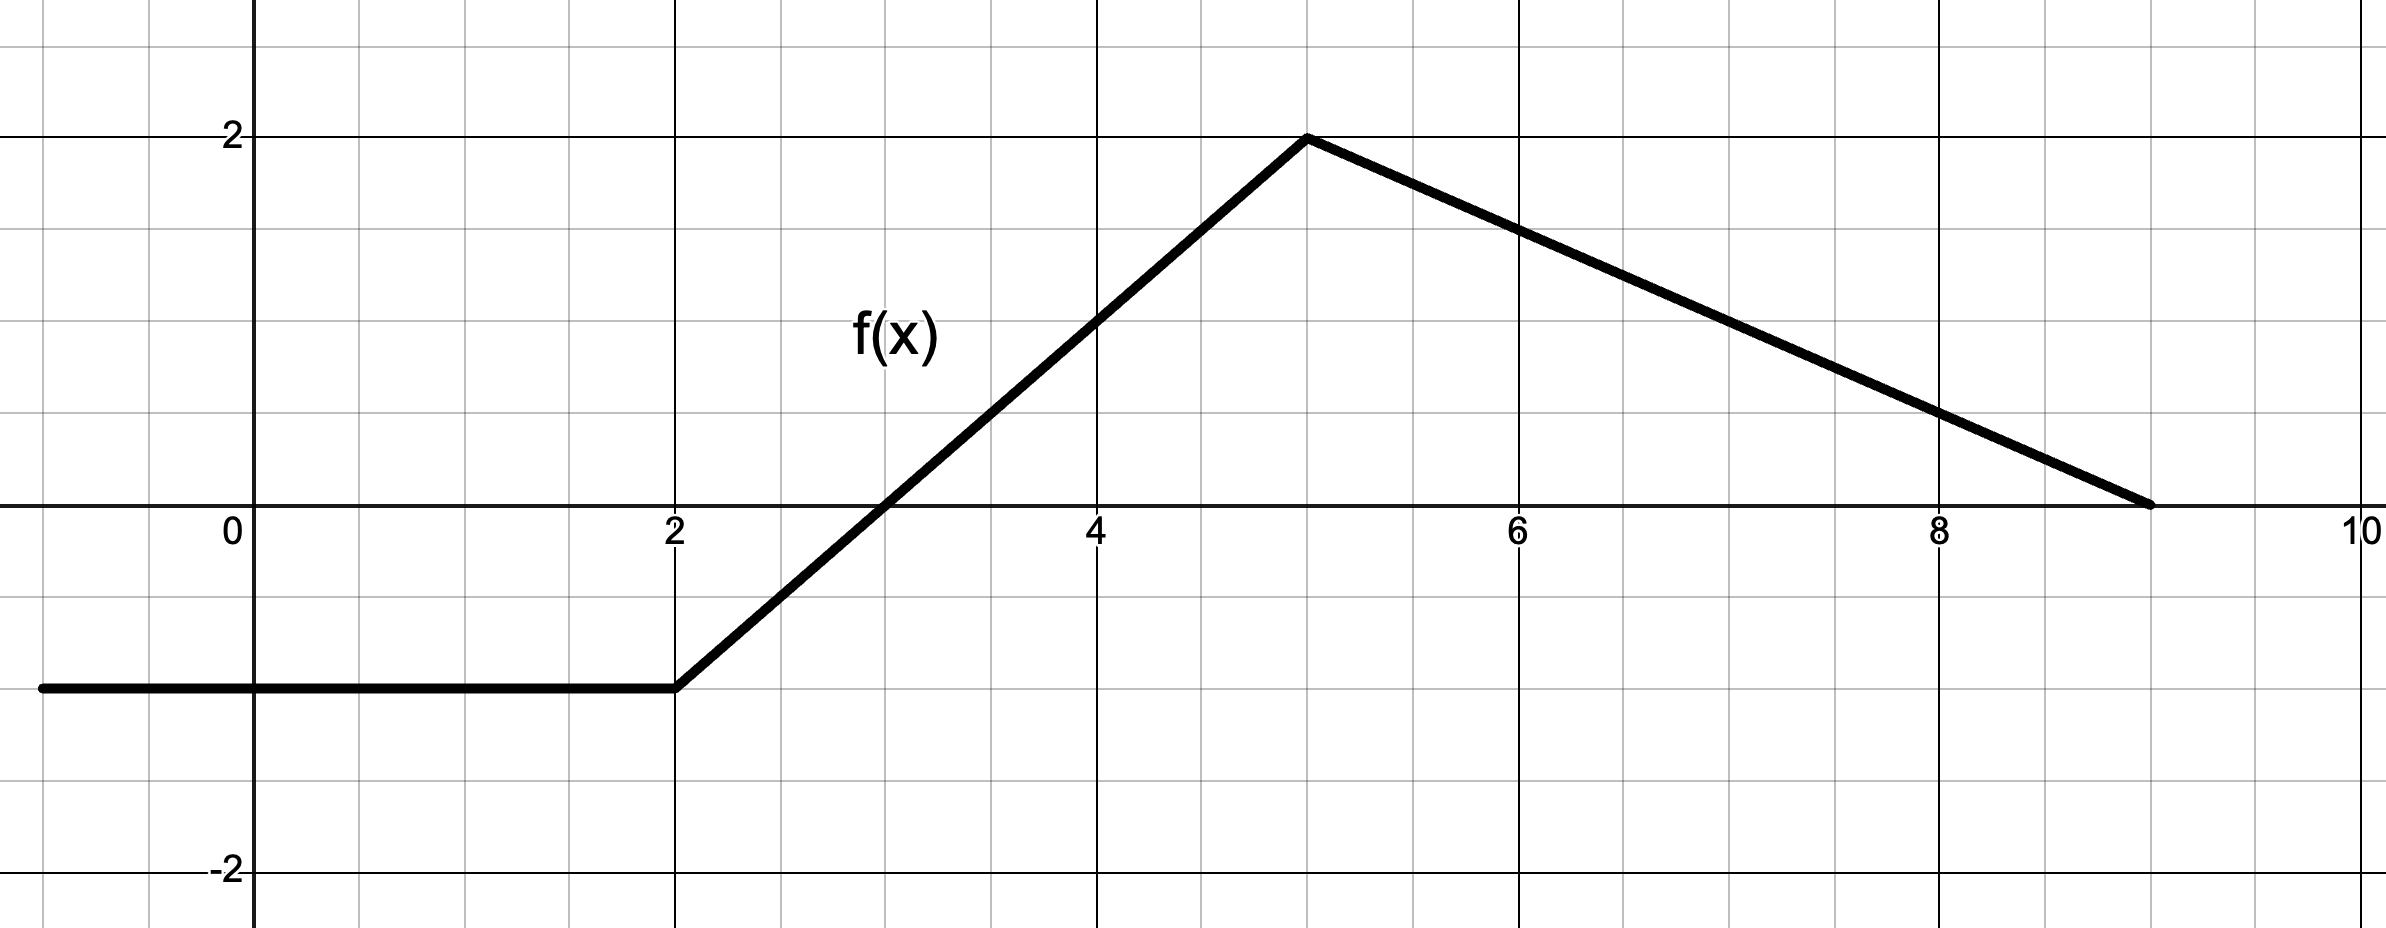
\includegraphics[width = \textwidth]{Support/Chapter 1 Graphics/1.5-Graphic3.png}
    \end{minipage} \hfill \begin{minipage}[t]{0.2\textwidth} \vspace{0pt}% 
        \def\arraystretch{1.4}
        $\begin{array}{|c|c|c|}
            \hline
            x & g(x) & g'(x) \\ \hline
            0 & -1 & 1 \\ \hline
            2 & 1 & 3 \\ \hline
            4 & 3 & 6 \\ \hline
            6 & 6 & 12 \\ \hline
            8 & 4 & 8 \\
            \hline
        \end{array}$
    \end{minipage} \\[11pt]

    (a) Find the equation of the line tangent to $f(x)$ at $x = 4$. \\[11pt]
    (b) Let $K$ be the function defined by $K(x) = h(f(x))$. Find $K'(3)$ \\[11pt]
    (c) Let $M$ be the function defined by $M(x) = g(x) \cdot f(x)$. Find $M'(6)$ \\[11pt]
    (d) Let $J$ be the function defined by $J(x) = \dfrac{g(x)}{h\left(\dfrac{1}{2}x\right)}$. Find $J'(8)$.
\end{tcolorbox}
\begin{tcolorbox}[solution]
    \textbf{Sol 1.5.5: } \\[11pt]
    (a) $f(4) = 1$ and $f'(4) = 1$. Therefore, the tangent line equation is \begin{align*}
        \boxed{y - 1 = 1(x - 4)}
    \end{align*}
    (b) \begin{align*}
        & h(x) = \ln \left(x^2 + 4\right) \\[11pt]
        & h'(x) = \dfrac{2x}{x^2 + 4} \\[11pt]
        & K(x) = h(f(x)) \therefore K = h'(f(x)) \cdot f'(x) \\[11pt]
        & K'(3) \begin{aligned}[t]
            & = h'(f(3)) \cdot f'(3) \\[11pt]
            & = h'(0) \cdot 1 \\[11pt]
            & = 0 \cdot 1 \\[11pt]
            & = \boxed{0}
        \end{aligned}
    \end{align*}
    (c) \begin{align*}
        & M(x) = g(x) \cdot f(x) \\[11pt]
        & M'(x) = g(x) \cdot f'(x) + f(x) \cdot g'(x) \\[11pt]
        & M'(6) \begin{aligned}[t]
            & = g(6) \cdot f'(6) + f(6) \cdot g'(6) \\[11pt]
            & = 6 \cdot \dfrac{1}{2} + 12 \cdot \dfrac{3}{2} \\[11pt]
            & = \boxed{15}
        \end{aligned}
    \end{align*}
    (d) \begin{align*}
        & J(x) = \dfrac{g(x)}{h\left(\dfrac{1}{2}x\right)} \\[11pt]
        & J'(x) = \dfrac{h\left(\dfrac{1}{2}x\right) \cdot g'(x) - g(x) \cdot h'\left(\dfrac{1}{2}x\right) \cdot \dfrac{1}{2}}{\left[h\left(\dfrac{1}{2}x\right)\right]^2} \\[11pt]
        & J'(8) \begin{aligned}[t]
            & = \dfrac{h(4) \cdot g'(8) - g(8) \cdot h'(4) \cdot \dfrac{1}{2}}{\left[h(4)\right]^2} \\[11pt]
            & = \boxed{\dfrac{8\ln 8 - \dfrac{4}{5}}{\ln^2 8}}
        \end{aligned}
    \end{align*}
\end{tcolorbox}

\newpage

\textbf{\large{1.5 Free Response Homework}} \par

1. Given the following table of values, find the indicated derivatives. \begin{align*}
    \arraycolsep=11pt\def\arraystretch{2.2}
    \begin{array}{|c|c|c|}
        \hline
        x & f(x) & f'(x) \\[5.5pt] \hline
        2 & 1 & 7 \\[5.5pt] \hline
        8 & 5 & -3 \\[5.5pt]
        \hline
    \end{array}
\end{align*}

\hspace{0.05\textwidth}\makebox[0.57\textwidth][l]{a) $g'(2)$, where $g(x) = [f(x)]^3$}\makebox[0.37\textwidth][l]{b) $h'2$, where $h(x) = f(x^3)$} \\[11pt]

2. The following table shows some values of $g(x), \; g'(x), \text{ and } h(x)$, where $h(x) = g^{-1}(x)$. \begin{align*}
    \arraycolsep=22pt\def\arraystretch{2.2} 
    \begin{array}{|c|c|c|c|c|}
        \hline
        x & g(x) & h(x) & g'(x) & h'(x) \\[5.5pt] \hline
        1 & 2 & 3 & \frac{1}{2} & \frac{1}{3} \\[5.5pt] \hline
        3 & 1 & 2 & -2 & \frac{1}{2} \\[5.5pt] 
        \hline
    \end{array}
\end{align*}

\hspace{0.05\textwidth}\makebox[0.57\textwidth][l]{a) Find $g'(1)$}\makebox[0.37\textwidth][l]{b) Find $h'(1)$} \\[11pt]

For problems 3 -- 14, refer to the values in the table below. \begin{align*}
    \arraycolsep=22pt\def\arraystretch{2.2} 
    \begin{array}{|c|c|c|c|c|}
        \hline
        x & f(x) & f'(x) & g(x) & g'(x) \\[5.5pt] \hline
        2 & 4 & -2 & 8 & 1 \\[5.5pt] \hline
        4 & 2 & 8 & 4 & 3 \\[5.5pt] \hline
        8 & 8 & -12 & 2 & 4 \\[5.5pt]
        \hline
    \end{array}
\end{align*}

\twoquestion{3. If $h(x) = f(g(x))$, find $h'(8)$}{4. If $h(x) = f(g(x))$, find $h'(2)$} \\[11pt]
\twoquestion{5. If $k(x) = g(f(x))$, find $k'(2)$}{6. If $m(x) = f(f(x))$, find $m'(4)$} \\[11pt]
\twoquestion{7. If $P_1(x) = f(x)g(x)$, find $P_1'(2)$}{8. If $P_1(x) = f(x)g(x)$, find $P_1'(8)$} \\[11pt]
\twoquestion{9. If $P_2(x) = f(2x)g(x)$, find $P_2'(2)$}{10. If $P_3(x) = f(x)g\left(\dfrac{1}{2}x\right)$, find $P_3'(4)$} \\[11pt]
\twoquestion{11. If $Q_1(x) = \dfrac{f(x)}{g(x)}$, find $Q_1'(2)$}{12. If $Q_2(x) = \dfrac{g(x)}{f(x)}$, find $Q_2'(8)$} \\[11pt]
\twoquestion{13. If $Q_3(x) = \dfrac{f(2x)}{g(x)}$, find $Q_3'(4)$}{14. If $Q_4(x) = \dfrac{g\left(\dfrac{1}{2}x\right)}{f(2x)}$, find $Q_4'(4)$} \\[11pt]

For problems 15 -- 26, the graphs of $f(x)$ and $g(x)$ are given below. \begin{center}
    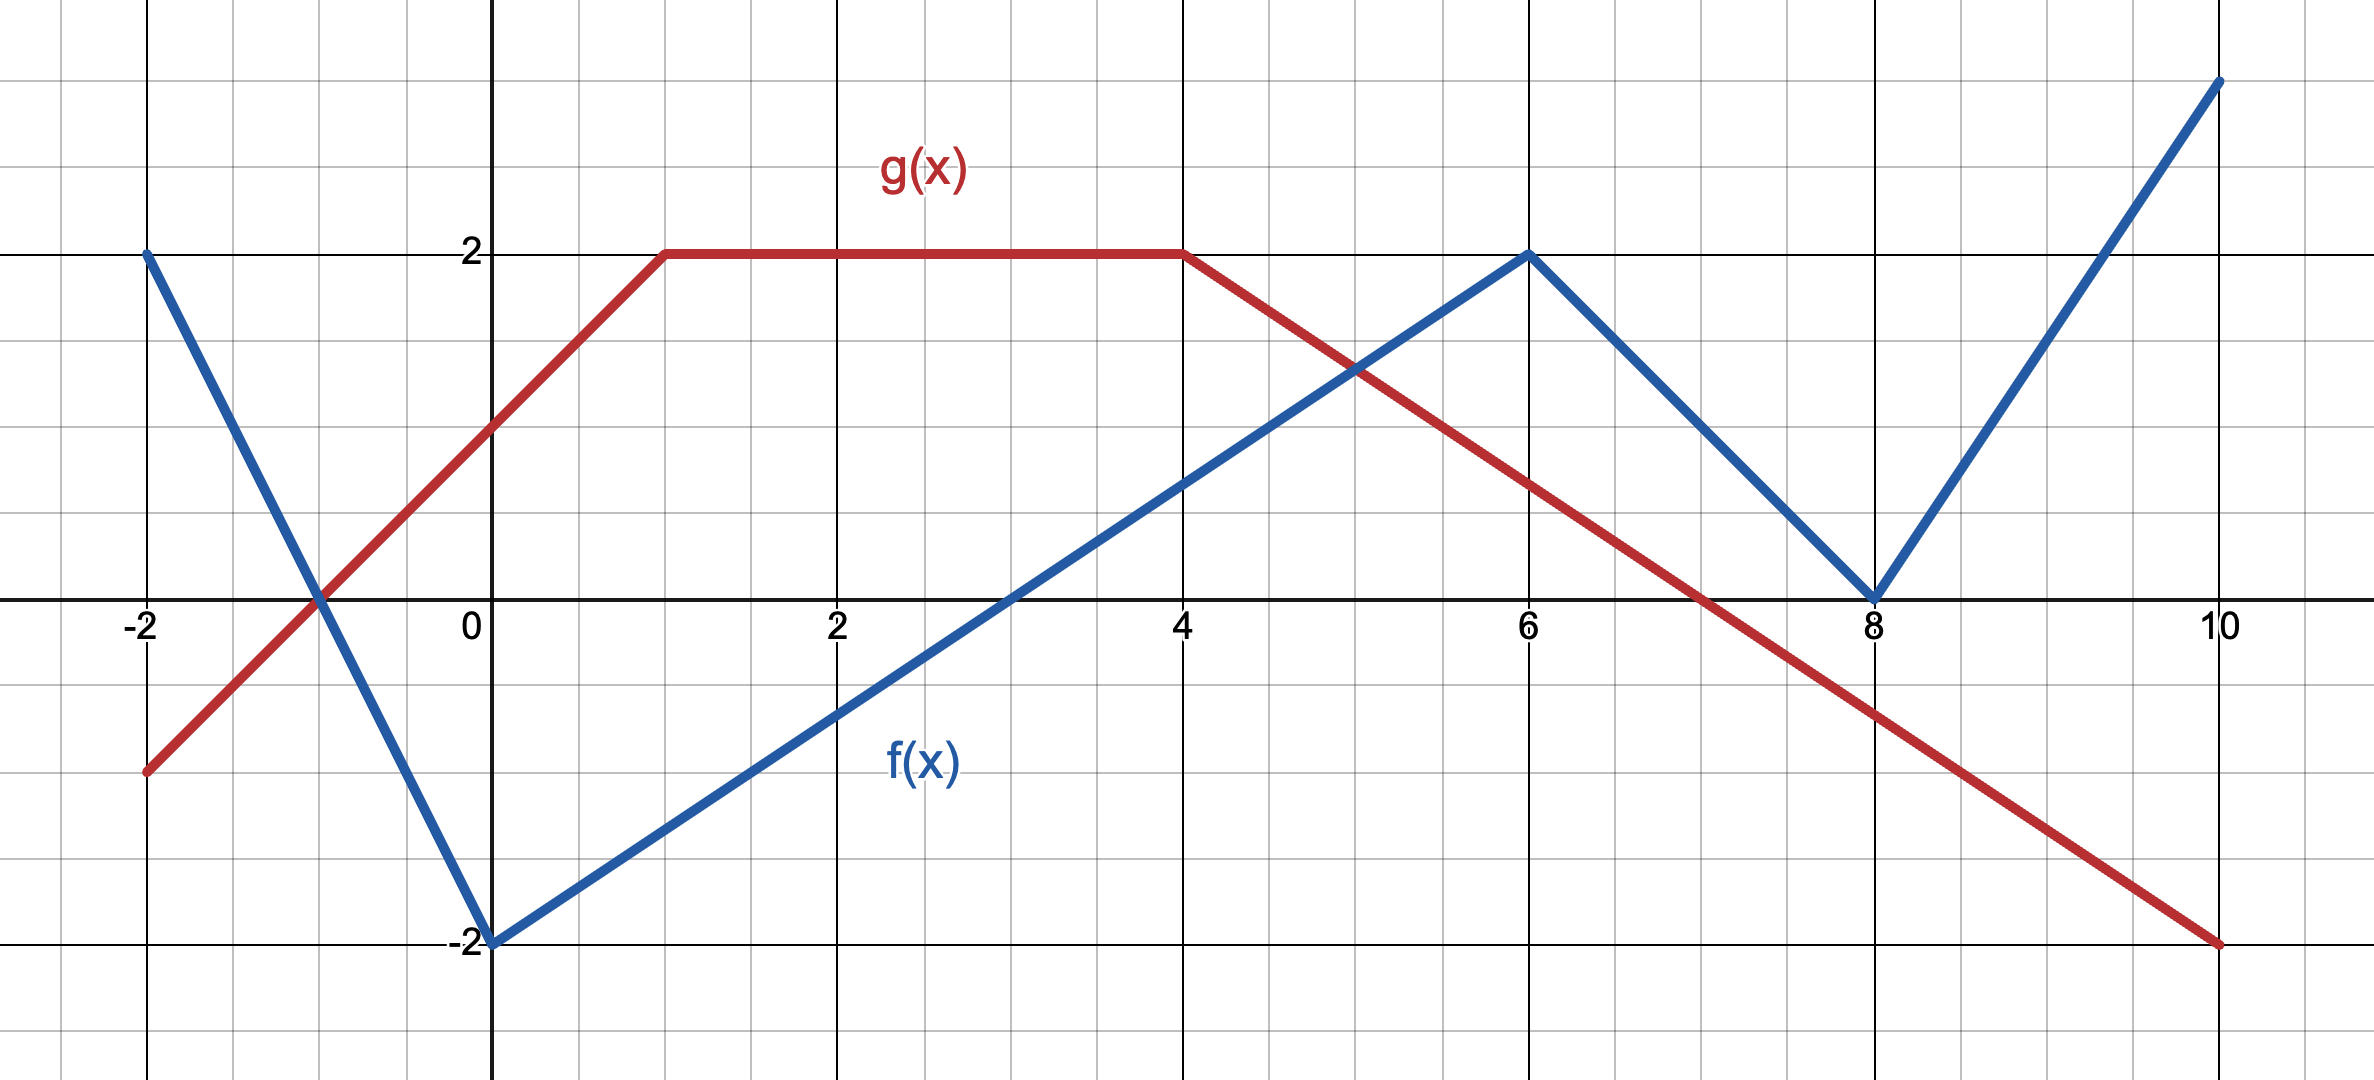
\includegraphics[width = \textwidth]{Support/Chapter 1 Graphics/1.5-Graphic4.png}
\end{center} 

\twoquestion{15. If $u = f(g(x))$, find $u'(2)$}{16. $v = g(f(x))$, find $v'(4)$} \\[11pt]
\twoquestion{17. If $w = g(g(x))$, find $w'(6)$}{18. If $t = f(f(x))$, find $t'(8)$} \\[11pt]
\twoquestion{19. If $P_1(x) = f(x)g(x)$, find $P_1'(2)$}{20. If $P_1(x) = f(x)g(x)$, find $P_1'(8)$} \\[11pt]
\twoquestion{21. If $P_2(x) = f(2x)g(x)$, find $P_2'(2)$}{10. If $P_3(x) = f(x)g\left(\dfrac{1}{2}x\right)$, find $P_3'(2)$} \\[11pt]
\twoquestion{23. If $Q_1(x) = \dfrac{f(x)}{g(x)}$, find $Q_1'(2)$}{24. If $Q_2(x) = \dfrac{g(x)}{f(x)}$, find $Q_2'(8)$} \\[11pt]
\twoquestion{25. If $Q_3(x) = \dfrac{f(2x)}{g(x)}$, find $Q_3'(4)$}{26. If $Q_4(x) = \dfrac{g\left(\dfrac{1}{2}x\right)}{f(2x)}$, find $Q_4'(4)$} \\[11pt]

\onequestion{27. Let $f(x)$ be the function whose graph is given below, and let $g(x)$ be a differentiable function with selected values for $g(x)$ and $g'(x)$ given in the table below.} \\
\begin{minipage}[t]{0.75\textwidth} \vspace{0pt}%
    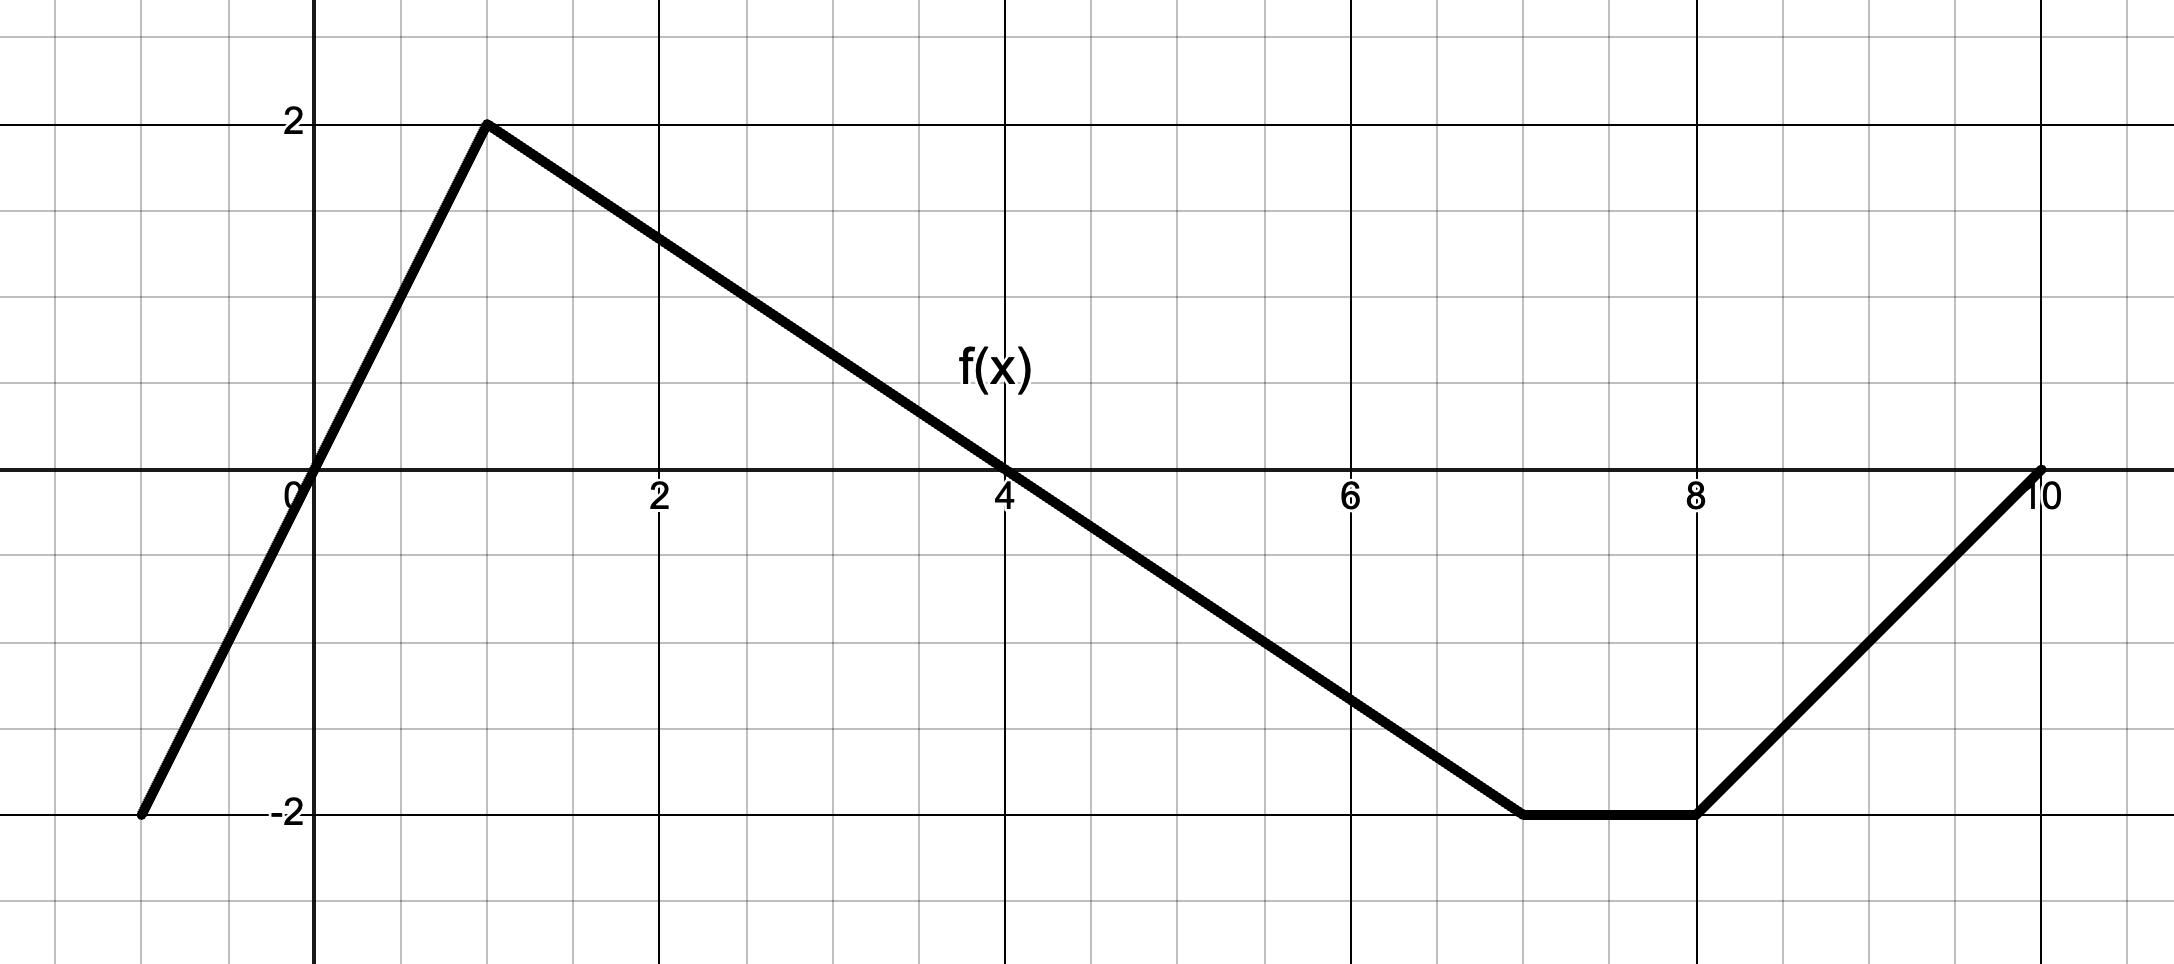
\includegraphics[width = \textwidth]{Support/Chapter 1 Graphics/1.5-Graphic5.png}
\end{minipage} \hfill \begin{minipage}[t]{0.2\textwidth} \vspace{11pt}% 
    \def\arraystretch{1.4}
    $\begin{array}{|c|c|c|}
        \hline
        x & g(x) & g'(x) \\ \hline
        0 & -1 & 1 \\ \hline
        2 & 1 & 3 \\ \hline
        4 & 3 & 6 \\ \hline
        6 & 6 & 12 \\ \hline
        8 & 4 & 8 \\
        \hline
    \end{array}$
\end{minipage} \\

(a) Find the equation of the line tangent to $f(x)$ at $x = 4$. \\[11pt]
(b) Let $K$ be the function defined by $K(x) = g(f(x))$. Find $K'(1)$. \\[11pt]
(c) Let $M$ be the function defined by $M(x) = g(x) \cdot f(x)$. Find $M'(4)$. \\[11pt]
(d) Let $J$ be the function defined by $J(x) = \dfrac{f(2x)}{g(x)}$. Find $J'(2)$. \\[11pt]

\onequestion{28. Let $f(x)$ be the function whose graph is given below, and let $g(x)$ be a differentiable function with selected values for $g(x)$ and $g'(x)$ given in the table below.} \\
\begin{minipage}[t]{0.75\textwidth} \vspace{0pt}%
    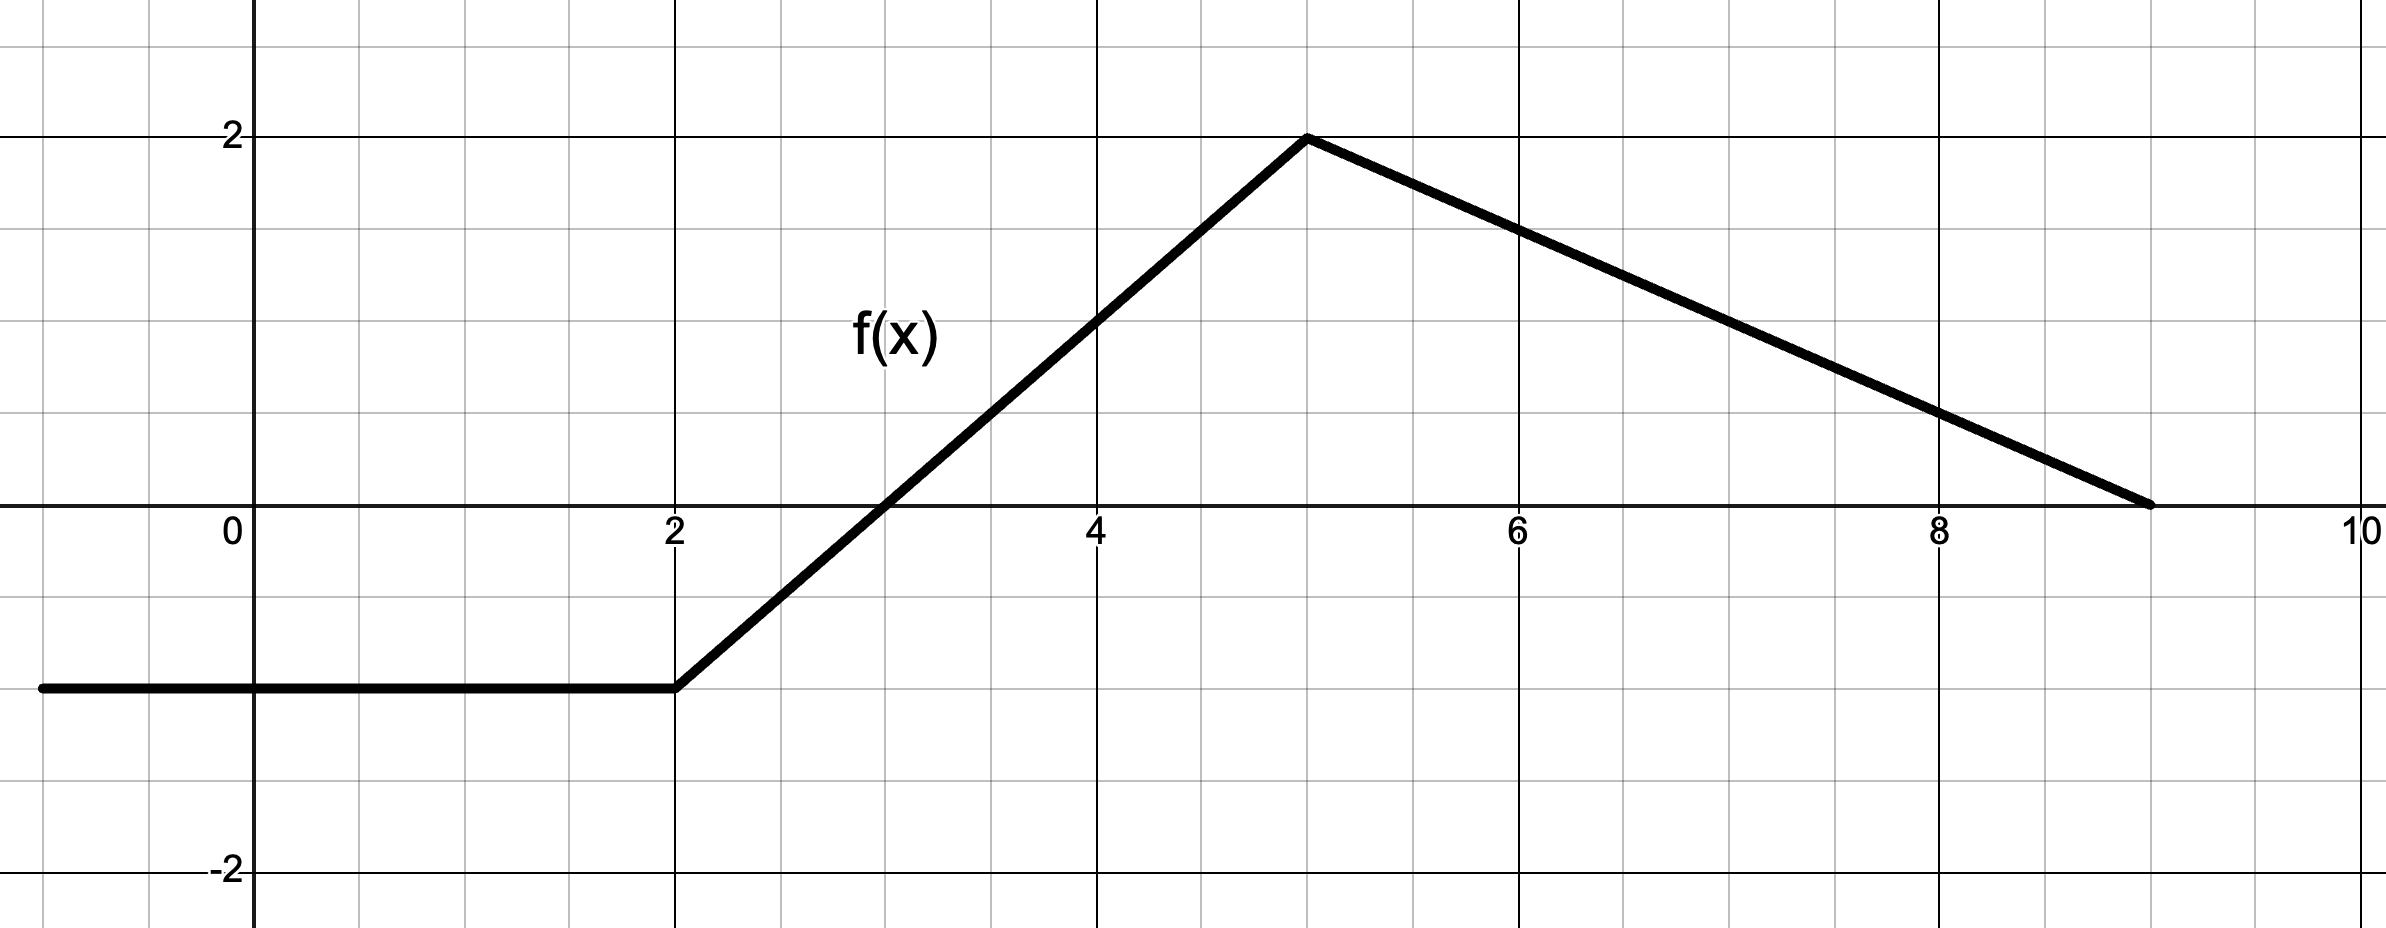
\includegraphics[width = \textwidth]{Support/Chapter 1 Graphics/1.5-Graphic3.png}
\end{minipage} \hfill \begin{minipage}[t]{0.2\textwidth} \vspace{0pt}% 
    \def\arraystretch{1.4}
    $\begin{array}{|c|c|c|}
        \hline
        x & g(x) & g'(x) \\ \hline
        0 & -1 & 1 \\ \hline
        2 & 1 & 3 \\ \hline
        4 & 3 & 6 \\ \hline
        6 & 6 & 12 \\ \hline
        8 & 4 & 8 \\
        \hline
    \end{array}$
\end{minipage} \\

(a) Find the equation of the line tangent to $g(x)$ at $x = 4$. \\[11pt]
(b) Let $K$ be the function defined by $K(x) = g(g(x))$. Find $K'(8)$. \\[11pt]
(c) Let $M$ be the function defined by $M(x) = g(x) \cdot f(x)$. Find $M'(4)$. \\[11pt]
(d) Let $J$ be the function defined by $J(x) = \dfrac{g(2x)}{f(x)}$. Find $J'(1)$. \\[11pt]

\onequestion{29. Let $f(x)$ be the function defined by $f(x) = 4x - x^3$, let $h(x)$ be the function whose graph is given below, and let $g(x)$ be a differentiable function with selected values of $g(x)$ and $g'(x)$ given in the table below.} \\
\begin{minipage}[t]{0.75\textwidth} \vspace{0pt}%
    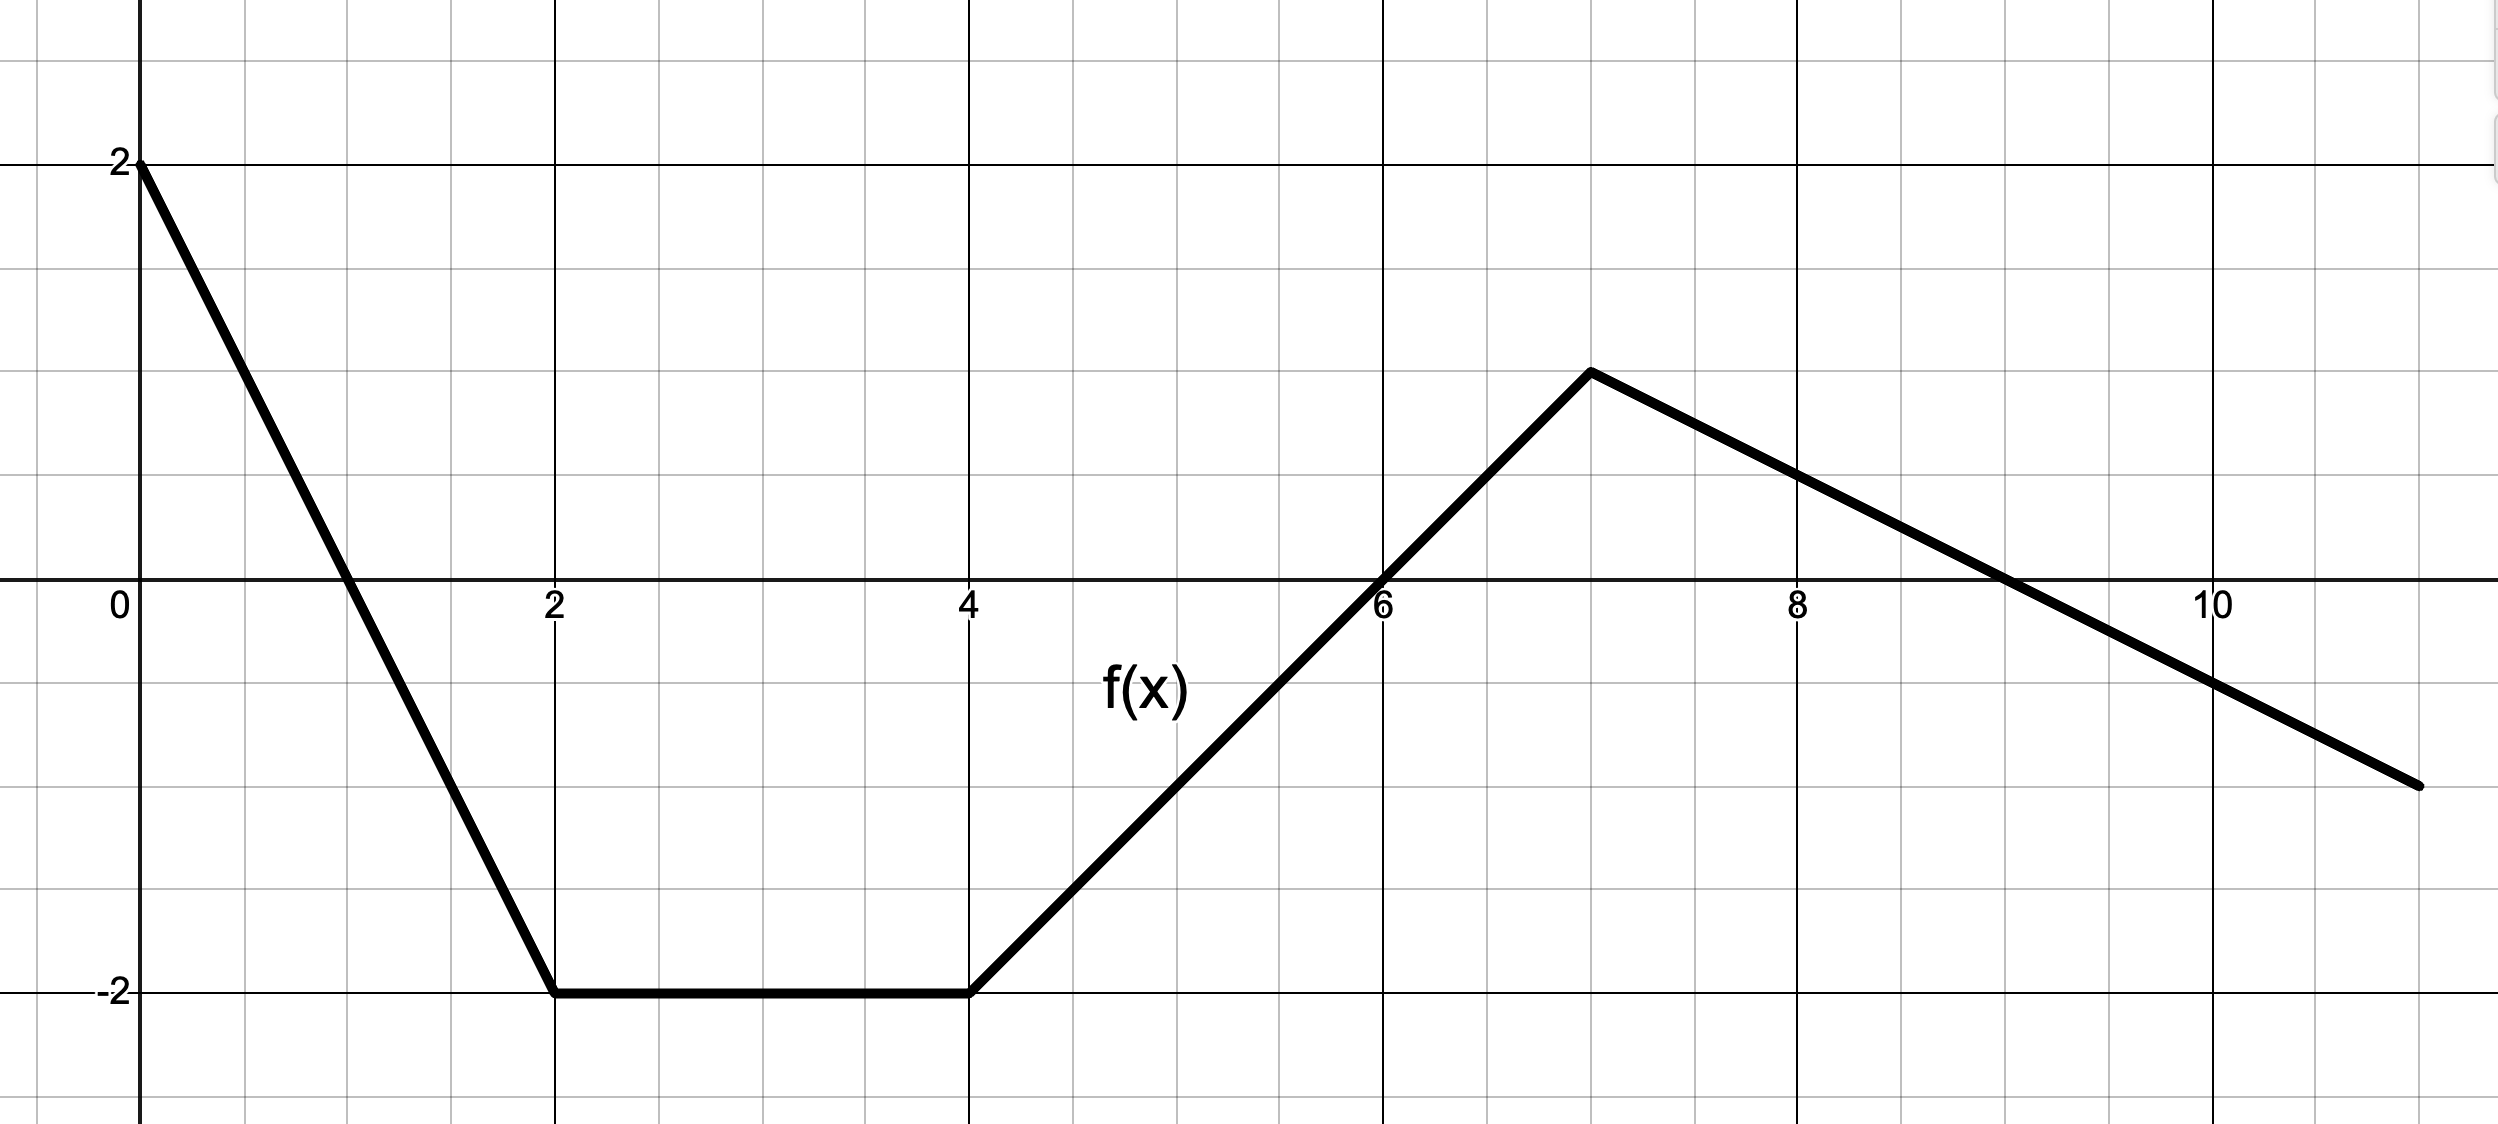
\includegraphics[width = \textwidth]{Support/Chapter 1 Graphics/1.5-Graphic6.png}
\end{minipage} \hfill \begin{minipage}[t]{0.2\textwidth} \vspace{11pt}% 
    \def\arraystretch{1.4}
    $\begin{array}{|c|c|c|}
        \hline
        x & g(x) & g'(x) \\ \hline
        0 & -1 & 1 \\ \hline
        2 & 1 & 3 \\ \hline
        4 & 3 & 6 \\ \hline
        6 & 6 & 12 \\ \hline
        8 & 4 & 8 \\
        \hline
    \end{array}$
\end{minipage} 

(a) Find the equation of the line tangent to $g(x)$ at $x = 4$. \\[11pt]
(b) Let $K$ be the function defined by $K(x) = h(f(x))$. Find $K'(1)$. \\[11pt]
(c) Let $M$ be the function defined by $M(x) = g(x) \cdot f(x)$. Find $M'(6)$. \\[11pt]
(d) Let $J$ be the function defined by $J(x) = \dfrac{g(x)}{f(x)}$. Find $J'(4)$. \\[11pt]

\onequestion{30. Let $h$ be the function defined by $h(x) = \sin (x) + e^{\cos (3x)}$, let f(x) be the function whose graph is given below, and let g(x) be a differentiable function with selected values of $g(x)$ and $g'(x)$ given in the table below.} \\
\begin{minipage}[t]{0.75\textwidth} \vspace{0pt}%
    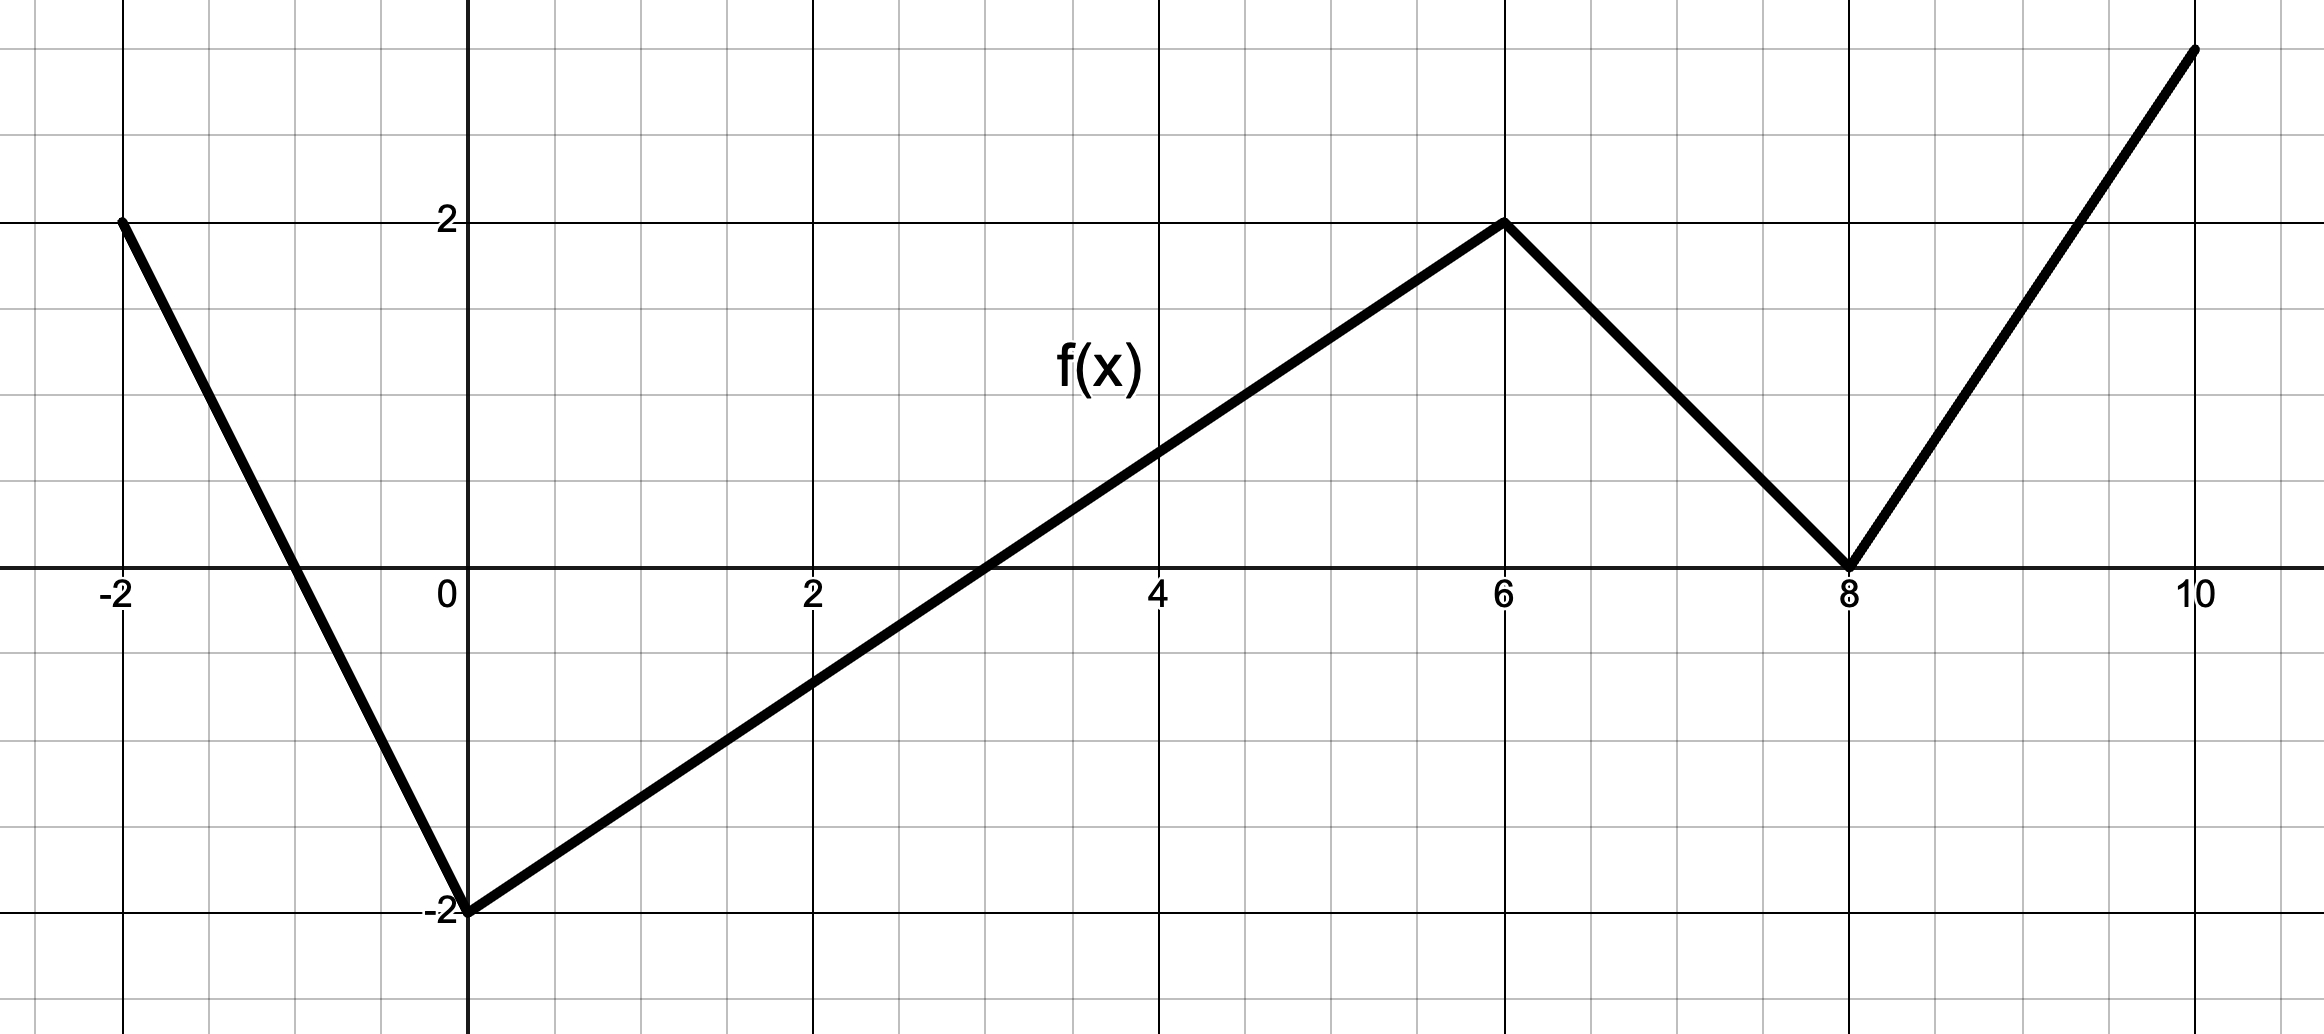
\includegraphics[width = \textwidth]{Support/Chapter 1 Graphics/1.5-Graphic7.png}
\end{minipage} \hfill \begin{minipage}[t]{0.2\textwidth} \vspace{11pt}% 
    \def\arraystretch{1.4}
    $\begin{array}{|c|c|c|}
        \hline
        x & g(x) & g'(x) \\ \hline
        -4 & 3 & 2 \\ \hline
        -2 & 5 & -1 \\ \hline
        0 & 7 & 0 \\ \hline
        2 & 5 & -1 \\ \hline
        4 & 3 & 2 \\
        \hline
    \end{array}$
\end{minipage} 

(a) Find the equation of the line tangent to $h(x)$ at $x = \dfrac{\pi}{2}$. \\[11pt]
(b) Let $K$ be the function defined by $K(x) = f(h(x))$. Find $K'\left(\dfrac{\pi}{2}\right)$. \\[11pt]
(c) Let $M$ be the function defined by $M(x) = f(x) \cdot g(x)$. Find $M'(0)$. \\[11pt]
(d) Let $J$ be the function defined by $J(x) = g(2x) \cdot f(x)$. Find $J'(2)$. \\[11pt]

\onequestion{31. \href{https://apcentral.collegeboard.org/media/pdf/ap-calculus-ab-frq-2017.pdf\#page=7}{{\text{\textcolor{blue}{2017 AP Calculus AB \#6}}}}} \\[11pt]

\textbf{\large{1.5 Multiple Choice Homework}} \par

\begin{questions}
    \question Let the function $f$ be differentiable on the interval $[0, 2.5]$ and $g$ be defined by $g(x) = f(f(x))$. Use the table to find $g'(1.5)$.
\end{questions}